\documentclass[11pt]{article}
\usepackage{fancyhdr}
\pagestyle{fancy}
\newcommand\course{ASTR 101}
\newcommand\hwnumber{2}
\newcommand\duedate{September 29, 2020}

\lhead{Oliver Tonnesen\\V00885732}
\chead{\textbf{\Large Lab \hwnumber{} Report}}
\rhead{\course\\\duedate}

\usepackage[
	backend=biber,
	url=true
]{biblatex}
\addbibresource{lab2.bib}
\usepackage{enumitem}
\usepackage{graphicx}
\usepackage{url}
\usepackage{pgfplots}
\pgfplotsset{width=10cm,compat=1.9}


\begin{document}
\section{Objective}
This lab exercise studies the creation, measurement, and interpretation of elements' spectral emissions, with a particular emphasis on potential applications in astronomy.


\section{Introduction}
Light behaves simultaneously as a particle and as a wave; in this lab we focus mainly on the wavelike nature of light.

As with all waves, light can be characterised by its \emph{wavelength}, the distance between any two peaks of a wave.
The wavelength of a light source determines its observed colour.
Shorter wavelengths appear closer to violet in colour, and longer wavelengths appear closer to red.
Wavelengths are often measured in nanometres (nm) or angstroms (\r{A}, where 1\r{A} = 0.1nm).

Most sources of light emit more than one single wavelength of light.
In these cases, much more insight into many of the light source's properties can be gained by studying its \emph{spectrum}, the measurement of the light's intensity at each different level of energy.

There are three broad categories of spectra: \emph{continuum spectra}, \emph{absorption spectra}, and \emph{emission spectra}.

Continuum spectra are characterised by a smooth distribution of wavelengths across the entire spectrum with no distinct bright or dark bars at any given wavelength.

Absorption spectra are similar to continuum spectra, but there are distinct dark bars of very low energy at specific wavelengths.
Absorption spectra are so named due to the fact that low energy electrons in atoms absorb energy at only specific wavelengths, so when a light emitting a continuous spectrum of light is observed through a cloud of gas for example, absorption lines corresponding to the gaseous element's electrons can be seen.

Emission spectra look like a collection of discrete spectral lines appearing only at particular wavelengths in the spectrum.
These spectra are so named since high energy electrons in atoms emit energy only at specific wavelengths, and so form an emission spectrum when observed.

Every element emits and absorbs a unique set of energy wavelengths.
We can use this fact to determine the presence of certain elements from the spectrum emitted by faraway galaxies, stars, hot gases, and other distant cosmic media.
We can also use these spectra, along with the \emph{Doppler effect} -- the uniform shift in wavelength due to the motion of the observed medium towards or away from us -- to determine objects' speeds.


\section{Observations, Tables, and Graphs}

\begin{table}[h]
\caption{Helium spectrum wavelengths and line positions.}
\renewcommand{\arraystretch}{1.5}
\begin{tabular}{| c | c | c | c |}
	\hline
	Line number & Wavelength (\r{A}) & Line position (pix) & Description\\ \hline
	-- & -- && Zero order image\\ \hline
	8 & 3889 & 238 & Deep violet\\ \hline
	7 & 4471 & 273 & Bright blue-violet\\ \hline
	6 & 4713 & 288 & Faint blue-violet\\ \hline
	5 & 4922 & 300 & Blue-green\\ \hline
	4 & 5016 & 307 & Blue-green\\ \hline
	3 & 5875 & 360 & Yellow\\ \hline
	2 & 6678 & 413 & Pale red\\ \hline
	1 & 7065 & 439 & Dark red\\
	\hline
\end{tabular}
\label{table:helium_spectrum}
\end{table}

\begin{figure}
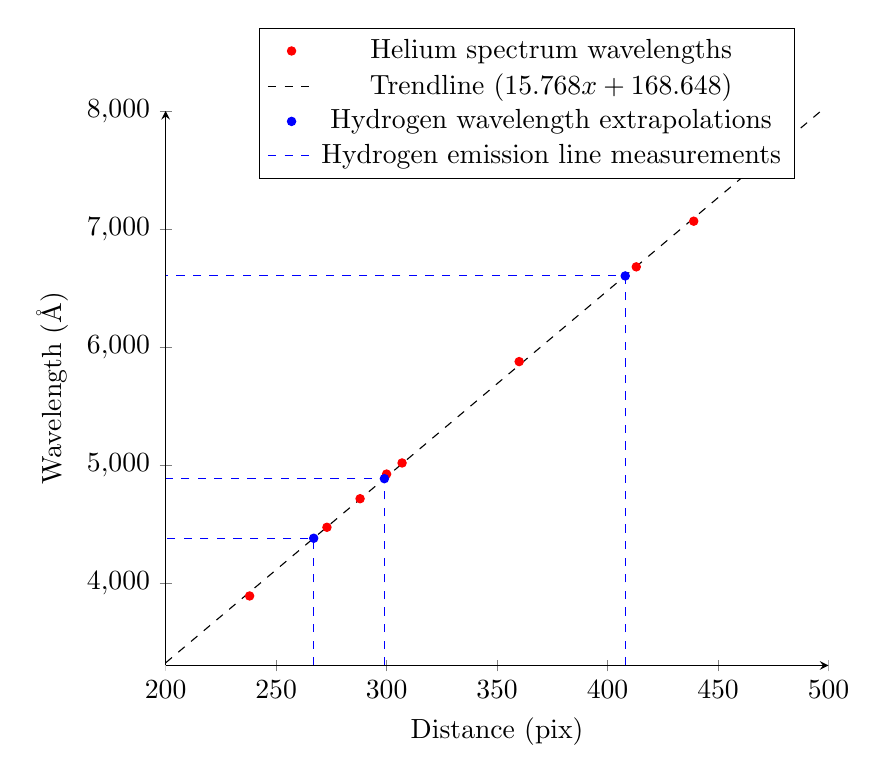
\begin{tikzpicture}
	\begin{axis}[
		axis lines=left,
		xlabel={Distance (pix)},
		ylabel={Wavelength (\r{A})},
		xmin=200, xmax=500,
		ymin=3300, ymax=8000,
		legend style={
			at={(0.95,1.15)},
		},
	]
	\addplot[
		only marks,
		mark size=1.5pt,
		color=red,
	] coordinates {(238,3889) (273,4471) (288,4713) (300,4922) (307,5016) (360,5875) (413,6678) (439,7065)};
	\addlegendentry{Helium spectrum wavelengths}
	\addplot [
		domain=200:500,
		style=dashed,
	] {15.768*x + 168.648};
	\addlegendentry{Trendline ($15.768x + 168.648$)}
	\addplot[
		only marks,
		mark size=1.5pt,
		color=blue,
		] coordinates {(267,4378) (299,4883) (408,6601)};
	\addlegendentry{Hydrogen wavelength extrapolations}
	\addplot+[
		mark=none,
		style=dashed,
		color=blue,
	] coordinates {(267,3300) (267,4378) (200,4378)};
	\addplot+[
		mark=none,
		style=dashed,
		color=blue,
	] coordinates {(299,3300) (299,4883) (200,4883)};
	\addplot+[
		mark=none,
		style=dashed,
		color=blue,
	] coordinates {(408,3300) (408,6601) (200,6601)};
	\addlegendentry{Hydrogen emission line measurements}
	\end{axis}
\end{tikzpicture}
\caption{A linear trendline is calculated from the values recorded in Table~\ref{table:helium_spectrum} and used to extrapolate the wavelengths of Hydrogen's visible spectral lines from their distance in pixels, as seen in Table~\ref{table:hydrogen_emission}.}
\label{graph:wavelengths}
\end{figure}

\begin{table}[h]
\caption{Hydrogen emission line measurements.}
\renewcommand{\arraystretch}{1.5}
\begin{tabular}{| c | c | c | c |}
	\hline
	Balmer line & Line position (pix) & Wavelength (\r{A}) & Description\\ \hline
	$H_\alpha$ & 408 & 6601 & Bright red\\ \hline
	$H_\beta$ & 299 & 4883 & Blue\\ \hline
	$H_\gamma$ & 267 & 4378 & Faint blue\\
	\hline
\end{tabular}
\label{table:hydrogen_emission}
\end{table}

\section{Answers}
\begin{enumerate}[label={\textbf{\emph{(\arabic*)}}}]

	\item % 1
Since the incandescent lamp emits a continuous spectrum, we expect to see a relatively uniform distribution of wavelengths of light.
The incandescent light emits mostly at the centre of the visible spectrum, so at low power the middle colours in the spectrograph are brighter than those to the outside.
At high power, the lamp produces enough light closer to the wavelengths of violet and red for these colours to become visible, but still mainly emits between these two ranges, causing the green and yellow wavelengths to remain the brightest colours seen through the spectrograph.

	\item % 2
The fluorescent lamp excites gas of a single element to produce light, and so we expect to see an emission spectrum corresponding to the element used in the lamp.
Light produced this way is not very pleasing to look at, so the gas tubes are covered in a fluorescent coating to diffuse the light and cause it to appear more white.
It is for this reason that we don't see a pure emission spectrum, but a combination of an emission spectrum superposed on a continuum spectrum.

	\item % 3
The following table identifies the six elements for which the spectra are shown in Figure 3 of lab 2 in the Lab Manual:
\begin{center}
\begin{tabular}{| c | c |}
	\hline
	Spectrum & Element\\ \hline
	1 & Sodium\\ \hline
	2 & Hydrogen\\ \hline
	3 & Oxygen\\ \hline
	4 & Nitrogen\\ \hline
	5 & Iron\\ \hline
	6 & Mercury\\
	\hline
\end{tabular}
\end{center}
\underline{Sodium}: Sodium's spectrum has a clump of violet to blue lines fading in from very dim to moderately bright, followed by a pair of lines -- one light green and one bright yellow.
The latter two lines are quite distinctive.
\newline
\underline{Hydrogen}: Hydrogen's spectrum has one dim violet, one dark blue, one bright light blue, and one bright red line, the last of which made this element very easy to determine, as it's the only line on the entire right half of the spectrograph.
\newline
\underline{Oxygen}: Oxygen's spectrum has a pair of lines -- one violet and one dark blue -- followed by three green lines and then a group of ten evenly distributed lines varying from yellow to red.
\newline
\underline{Nitrogen}: Nitrogen's spectrum has one very bright violet line, four very light blue lines, two green lines, four yellow lines, and five very bright red lines.
\newline
\underline{Iron}: Iron's spectrum is a \emph{very} dense set of lines all the way from violet to red.
In some parts, it almost looks like an absorption spectrum because of how dense the spectral lines are.
\newline
\underline{Mercury}: Mercury's spectrum is very dense close to the centre of the visible spectrum (around green to yellow).
I has a very distinctive pair of orange lines followed by a pair of red lines very close to the infrared range.

	\item % 4
Below is a sketch of the emission spectrum of Lithium:
\newline
\newline

\includegraphics[scale=0.4]{Li.png}

	\item % 5
These absorption lines are referred to as Fraunhofer lines, after physicist Joseph von Fraunhofer~\cite{britannica-fraunhofer}.
These lines correspond to the absorption spectra of the gases in the Sun.

	\item % 6
Two of the elements in the Sun that cause these absorption lines are Oxygen and Iron.

	\item % 7
The presence of these heavier elements implies that the Sun is relatively young, and that it was potentially created by a nearby supernova~\cite{spacecom}.

	\item % 8
The peak wavelength of Betelgeuse is approximately 830nm, putting its primary emission in the infrared range of the electromagnetic spectrum.
Thus we expect that Betelgeuse should have a deep red colour.

	\item % 9
Betelgeuse has spectral class M2~\cite{stellardb-betelgeuse} -- red -- so our prediction was accurate.

	\item % 10
Sirius' peak wavelength is approximately 290nm, well into the ultraviolet range of the electromagnetic spectrum.
Thus we expect that Sirius should have a bright blue or white colour.

	\item % 11
Sirius has spectral class A1~\cite{stellardb-sirius} -- white -- so our prediction was accurate.

	\item % 12
If a star's spectrum peaked in the green region of the visual spectrum, its peak wavelength would be somewhere around 500nm, and it would be slightly yellow -- perhaps closer to white -- since it emits most of the visual spectrum (very similarly to the Sun).

	\item % 13
If a planet has an atmosphere, then we can measure its host star's spectrum after passing through it~\cite{phys-atmosphere-spec}.
The gases in the planet's atmosphere will absorb certain wavelengths of the star's spectrum.
This, paired with prior knowledge of the star's own absorption spectrum allow us to very accurately measure the composition of gas in the planet's atmosphere.
This method of detecting planets is challenging due to fact that the star and the planet have to be positioned in line with the spectrograph so that the star's light can pass through the planet's atmosphere before travelling to Earth.

	\item % 14
$H_\alpha = 6601$\r{A}, $H_\beta = 4883$\r{A}, and $H_\gamma = 4378$\r{A}.
Please refer to Figure~\ref{graph:wavelengths} to see how these values were obtained.

	\item % 15
$H_\alpha$: 38\r{A}, $H_\beta$: 22\r{A}, and $H_\gamma$: 38\r{A}.
The discrepancies are all quite small (less than 1\% error), but that of $H_\beta$ is smaller than that of $H_\alpha$ and $H_\gamma$.

	\item % 16
Human error in the measurement taken in GIMP is likely the cause of the above error, although uncertainly due to the thickness of the spectral lines in the image is another potential source of the error.
\end{enumerate}


\section{Discussion}
This lab exercise demonstrated how to measure and observe the spectra of elements and light sources.
We saw how to extrapolate from known data to determine the presence of elements in a light source's spectrum.

When measuring Hydrogen's Balmer lines, we saw less than a 1\% difference between the measured and the expected wavelengths.
This discrepancy is likely due to human error in taking the measurement from the image.


\section{Conclusion}
In this lab exercise, we learned how to interpret these spectra, and how they are affected by variables such as temperature, distance, and motion.
Additionally, we saw how astronomical spectroscopy can be used to determine such properties as elemental composition and speed in faraway cosmic objects.

\printbibliography

\end{document}
